\section{IAdapter}

IAdapter is a JMeter Plugin to perform evolutionary load, performance or stress tests. JMeter is a desktop application, designed to test and measure the performance and functional behavior of applications \cite{Nevedrov2007}.

The IAdapter plugin makes it possible to create a generative model that evolves during the test. The IAdapter model uses Genetic Algorithm, Tabu Search and Simulated Annealing in two different approaches.  The first approach uses the three algorithms independently and the second approach uses the three algorithms collaboratively (Hybrid Metaheuristic approach).

In the first approach , the algorithms do not share their best individuals among themselves. Each algorithm evolves in a separate way (Fig. \ref{fig:firstaproach}). The second approach use the algorithms in a collaborative mode (Hybrid Metaheuristic). In this approach, the three algorithms share their best individuals found (Fig. \ref{fig:secondapproach}).

The next subsections present details about the used metaheuristcs algorithms (genotype representation and fitnesse function) and the IAdapter components.

\begin{figure}[h]
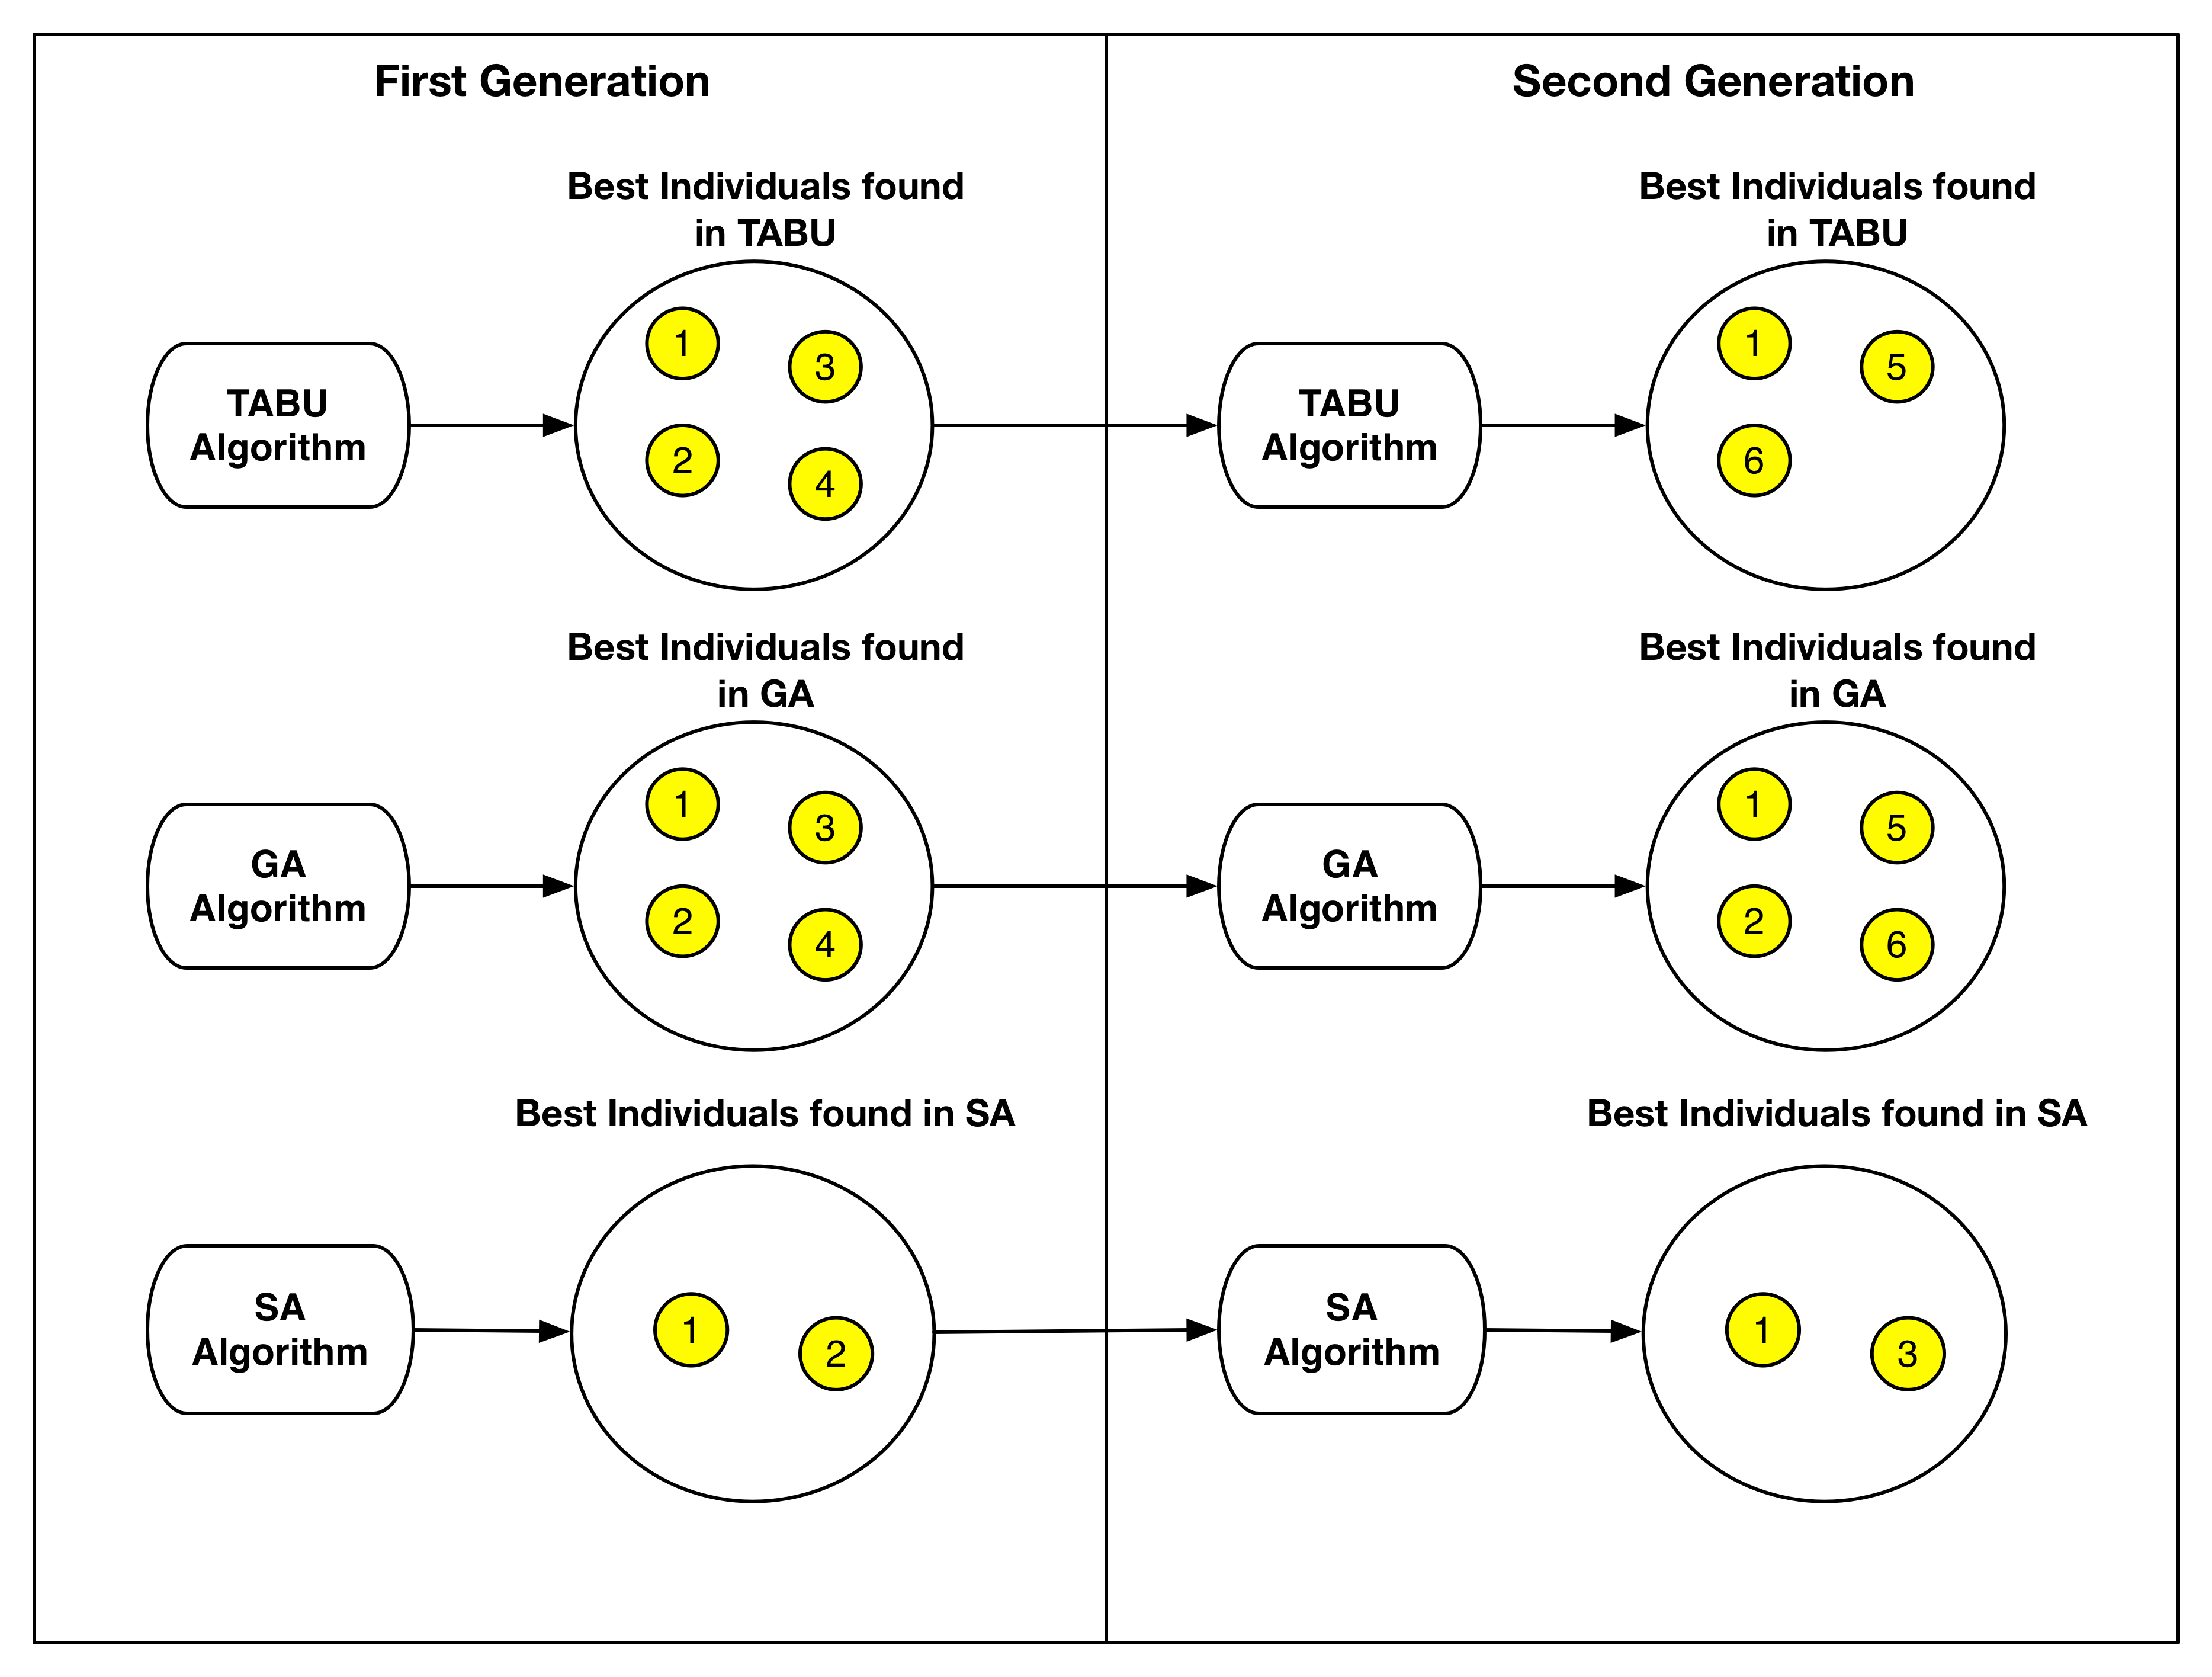
\includegraphics[width=0.5\textwidth]{./images/independ.png}
\caption{Use of the algorithms independently}
\label{fig:firstaproach}
\end{figure}
\begin{figure}
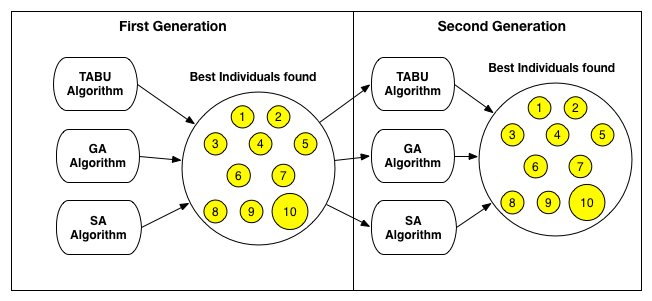
\includegraphics[width=0.5\textwidth]{./images/collaborative.png}
\caption{Use of the  algorithms collaboratively}
\label{fig:secondapproach}
\end{figure}

\subsection{Genotype representation}

The Genotype representation is composed by a linear vector with 23 genes. The first gene represents the name of individual. The second gene presents the  algorithm (Genetic Algorithm, Simulated Annealing or Tabu Search) used by the individual. The third gene represents the type of test (Load, Stress or Performance). Next genes represent 10 scenarios and their numbers of users. Each scenario is an atomic operation, the scenario must log in the application, run the task goal and undo any changes performed, returning the application to it's original state. 

The Fig. \ref{fig:genomarepresentation} presents the genome representation and  a example using the crossover operation. In the example, the genotype 1 has the Login scenario with 2 users; the Form scenario with 0 users and the Search scenario with 3 users. The genotype 2 has the Delete scenario with 10 users; the Search scenario with 0 users and the Include scenario with 5 users. After the crossover operation, We obtain a genotype with  Login scenario with 2 users; the Search scenario with 0 users and the Include scenario with 5 users.

\begin{figure}[h]
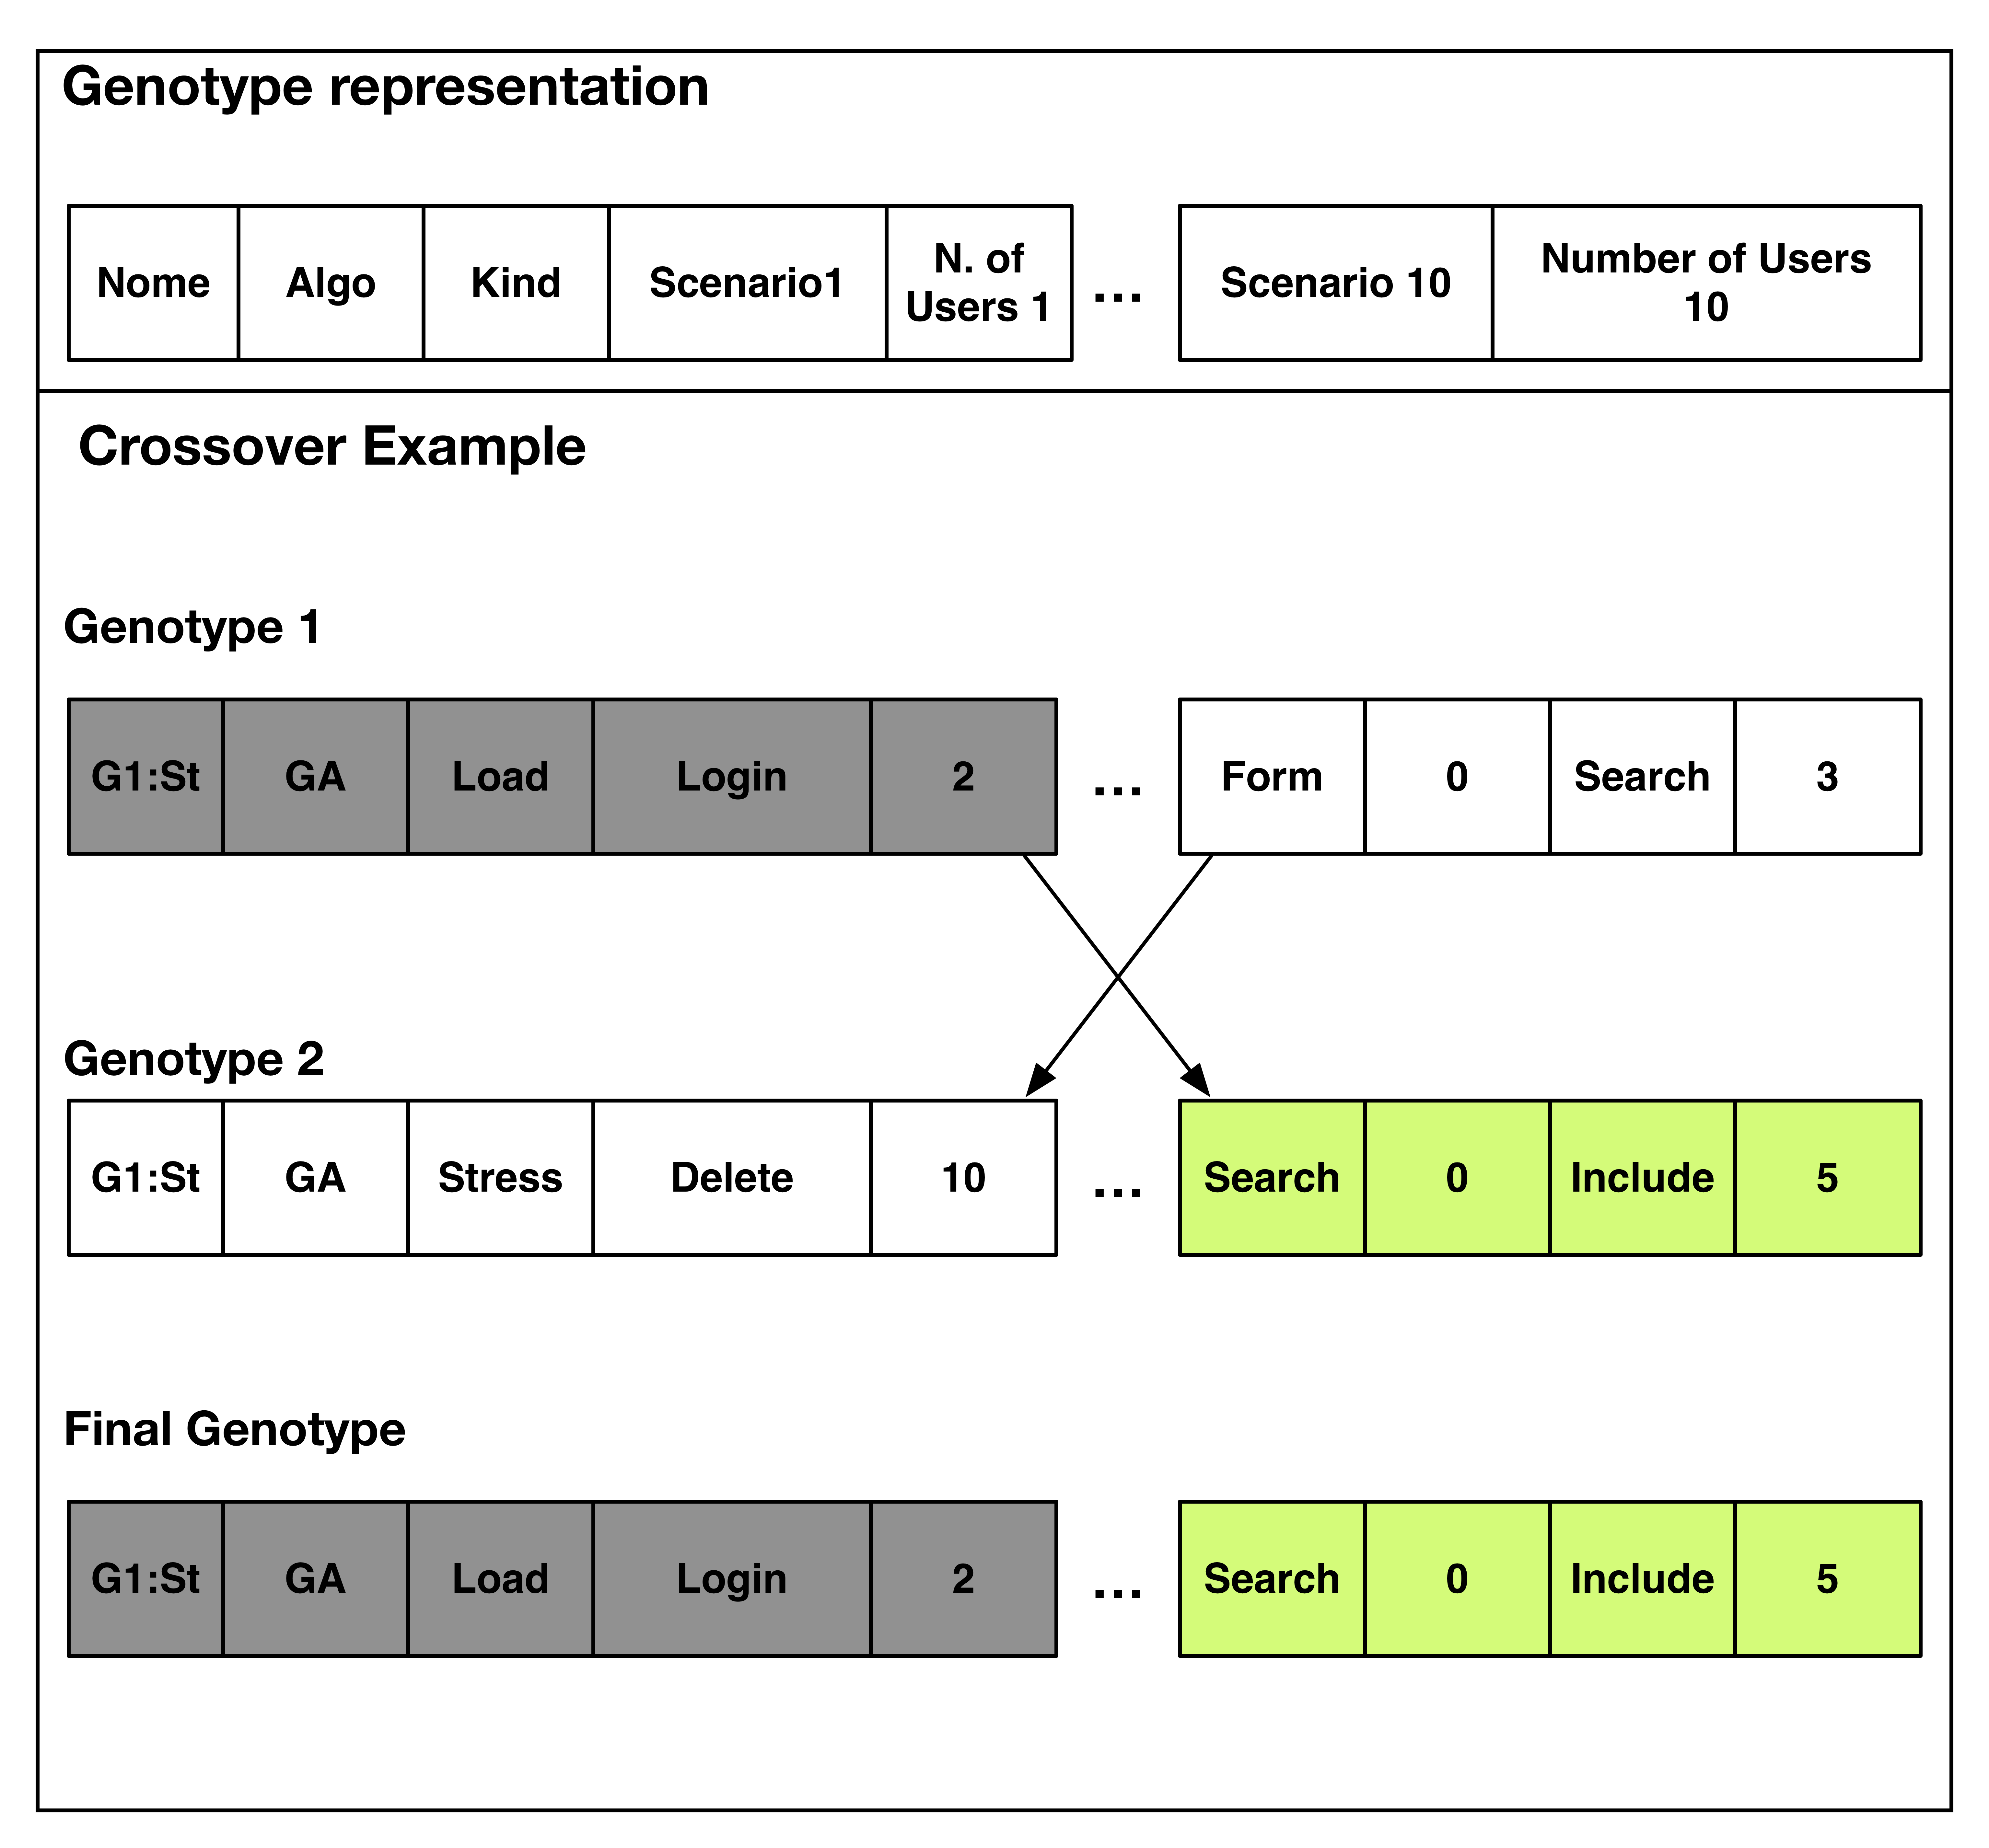
\includegraphics[width=0.5\textwidth]{./images/genomerepresentation.png}
\caption{Genotype representation and crossover example}
\label{fig:genomarepresentation}
\end{figure}

The Fig. \ref{fig:neighbourtaby} shows the strategy used by the IAdapter to obtain the genotype of the neighbours for the Tabu Search and Simulated Annealing algorithms.  The neighbours are obtained by the modification of a single cromossome (scenario or  number of users) in the genotype.

\begin{figure}[h]
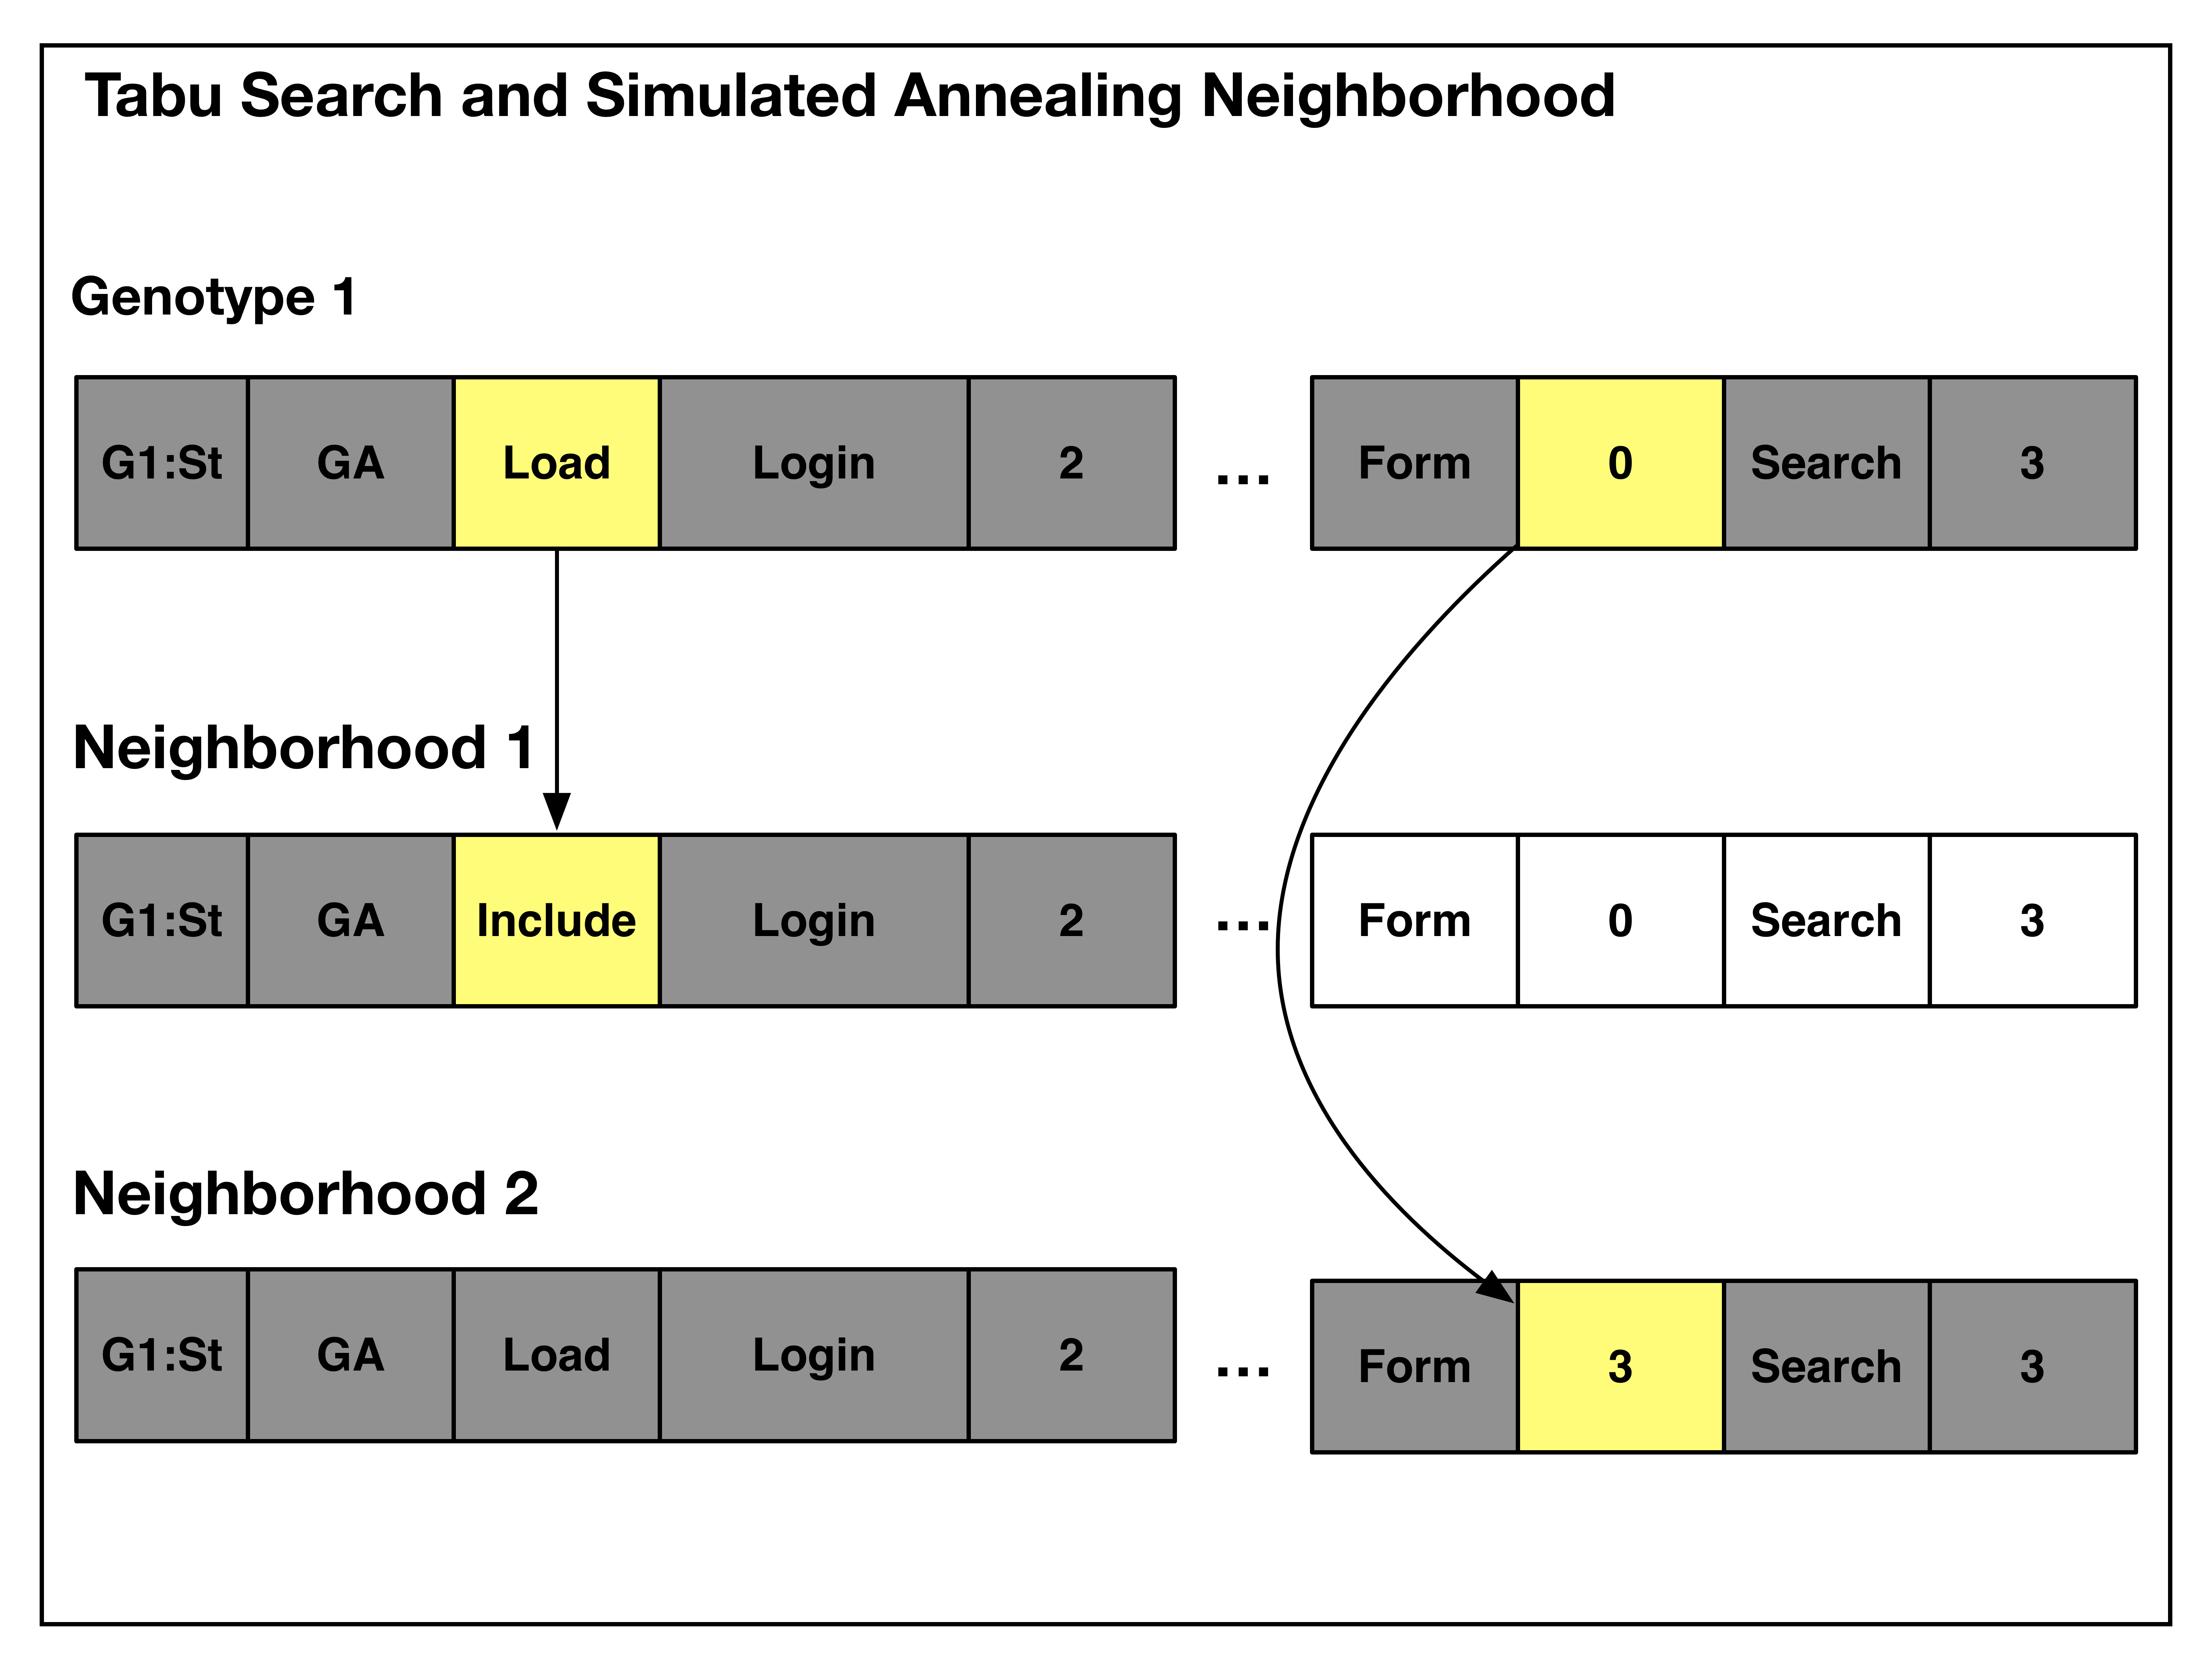
\includegraphics[width=0.5\textwidth]{./images/TabuNE.png}
\caption{Tabu Search and Simulated Annealing neighbour strategy}
\label{fig:neighbourtaby}
\end{figure}


\subsection{Objective (Fitnesse) Function}

The IAdapter is a tool to be used with the independent testing teams in various situations where the team has no direct access to the environment where the application under test was installed. Therefore,  The IAdapter uses a measurement approach to the definition of the fitnesse function. The fitnesse function applied to IAdapter solution is governed by the following equation:

\begin{equation}
\begin{aligned}
fit=90percentileweigth* 90percentiletime\\
+80percentileweigth*80percentiletime\\+
70percentileweigth*70percentiletime+\\
maxResponseWeigth*maxResponseTime+\\
numberOfUsersWeigth*numberOfUsers-penalty
\end{aligned}
\end{equation}

The IAdapter's fitnesse function uses a series of adaptable user-defined weights ( 90percentileweigth, 80percentileweigth,  70percentileweigth, maxResponseWeigth and numberOfUsersWeigth). These weights make it possible to customize the search plugin functionality. The penalty is applied when a application under test responds in a longer time than the level of service.

\subsection{IAdapter Components}

The JMeter have components organized  in a hierarchical manner. The IAdapter plugin provides three main components: WorkLoadThreadGroup, WorkLoadSaver, and WorkLoadController.
 
The WorkLoadThreadGroup is a component that creates an initial population and configure the algorithms used in IAdapter . The Fig. \ref{fig:tela1iadapter} presents the main screen of the WorkLoadThreadGroup component. The component has a name \ding{202}, a set of configuration tabs \ding{203}, a list of individuals by generation \ding{204}, a button to generate an initial population \ding{205} and a button to export the results \ding{206}.

\begin{figure}[h]
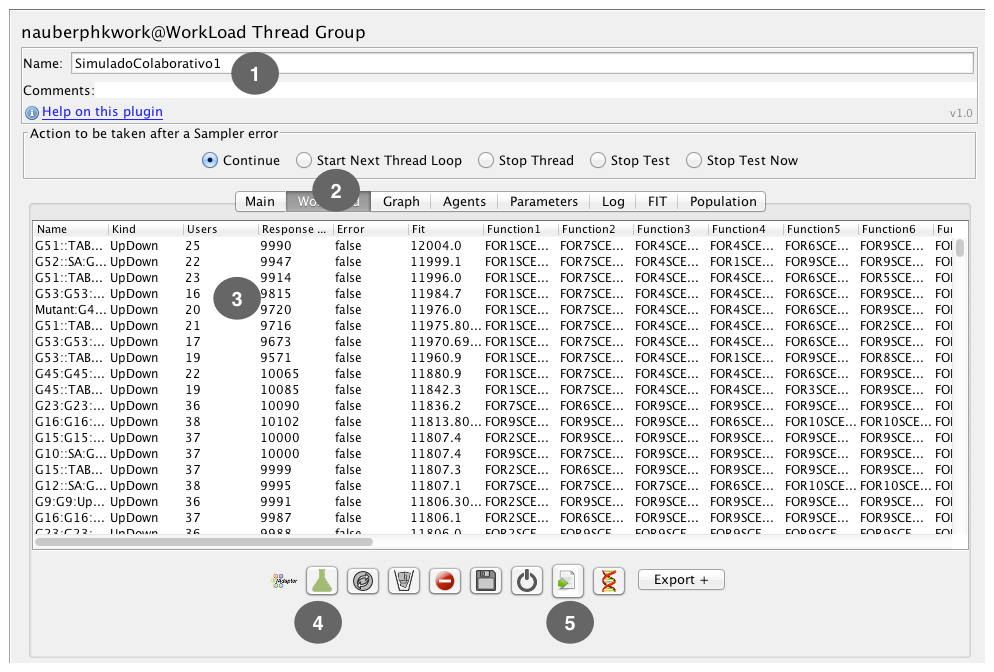
\includegraphics[width=0.5\textwidth]{./images/tela1iadapter.png}
\caption{WorkLoadThreadGroup component}
\label{fig:tela1iadapter}
\end{figure}

The WorkLoadSaver component is responsible for saving all data in the database. The operation of the component only requires its inclusion in the test script.

The WorkLoadController represents a scenario of test. The WorkLoadController represents a scenario of test. All actions necessary to test a application should be included in this component. All instance of the component need to login in the application under test and return the application to it's original state.